\documentclass[12pt,a4paper]{article}
\usepackage[utf8]{inputenc}
\usepackage[T1]{fontenc}
\usepackage{amsmath}
\usepackage{amsfonts}
\usepackage{amssymb}
\usepackage{graphicx}
\usepackage[indonesian]{babel}
\usepackage[left=2.00cm, right=2.00cm, top=2.00cm, bottom=2.00cm]{geometry}
\usepackage{float} 

\title{Tugas 14 - Pengolahan Sinyal Digital\\
	Disain Filter Digital IIR}

% remove spacing around date:
\usepackage{titling}
\predate{}
\postdate{}
\date{}

\begin{document}
	\maketitle
	\date{}
	\begin{enumerate}
		\item Diketahui suatu filter analog yang mana input $ x_a(t) $ dan output $ y_a(t) $ saling berkaitan dalam persamaan linear constant coefficient differential berikut:
		
		\[ \frac{dy_a(t)}{dt} + 0.9 y_a(t) = x_a(t) \]
		
		Filter digital didapatkan dengan cara mengganti turunan pertama dengan forward diference pertama sehingga
		
		\[ \left[ \frac{y(n+1) - y(n)}{T} \right] + 0.9 y(n) = x(n)  \]
		
		Asumsikan filter digital ini adalah kausal
		\begin{enumerate}
			\item Tentukan dan gambarkan magnitude dari frequency response analog filternya.\\
			\textbf{Jawaban:} Dengan melakukan transformasi Laplace terhadap kedua sisi dari persamaan diferensial, kita dapatkan:

			\begin{figure}[H]
				\centering
				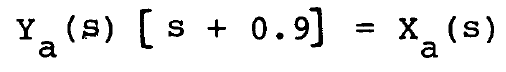
\includegraphics[width=0.3\linewidth]{img/img01}
			\end{figure}
			
			atau
			
			\begin{figure}[H]
				\centering
				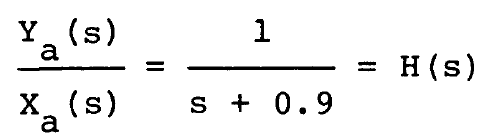
\includegraphics[width=0.3\linewidth]{img/img02}
			\end{figure}
			
			maka
			
			\begin{figure}[H]
				\centering
				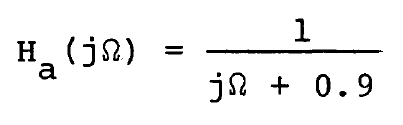
\includegraphics[width=0.3\linewidth]{img/img03}
			\end{figure}
		
			dan
			
			\begin{figure}[H]
				\centering
				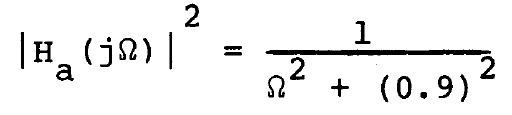
\includegraphics[width=0.3\linewidth]{img/img04}
			\end{figure}
			
			dan grafiknya
			
			\begin{figure}[H]
				\centering
				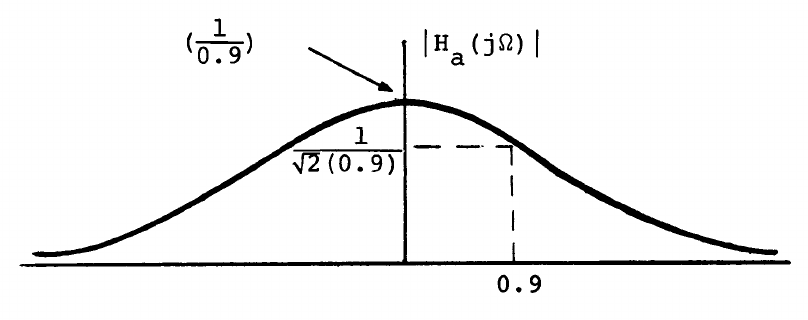
\includegraphics[width=0.7\linewidth]{img/img05}
			\end{figure}
		
			\item\label{b} Tentukan dan gambarkan magnitude dari frequency response digital filter untuk $ T = 10/9 $.\\
			\textbf{Jawaban:} Dengan melakukan transformasi z terhadap kedua sisi persamaan beda, kita dapatkan:
			
			\begin{figure}[H]
				\centering
				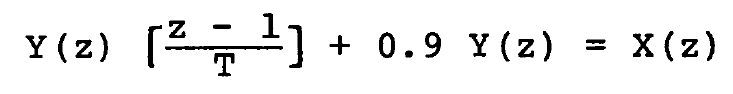
\includegraphics[width=0.5\linewidth]{img/img06}
			\end{figure}
			
			atau
			
			\begin{figure}[H]
				\centering
				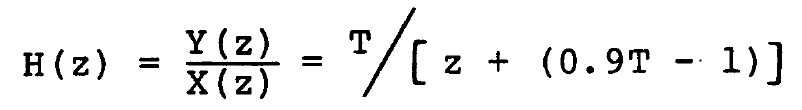
\includegraphics[width=0.5\linewidth]{img/img07}
			\end{figure}
		
			dengan $ T = \frac{10}{9} $ maka,
			
			\begin{figure}[H]
				\centering
				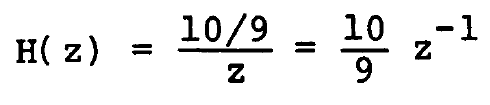
\includegraphics[width=0.3\linewidth]{img/img08}
			\end{figure}
		
			dan
			
			\begin{figure}[H]
				\centering
				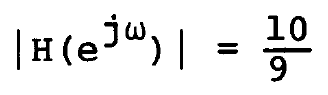
\includegraphics[width=0.2\linewidth]{img/img09}
			\end{figure}
			
			dengan nilai T tersebut frekuensi responsenya konstan, independent frekuensi sangat berbeda dengan filter analog, yang mana merupakan lowpass filter. Di sini kita lakukan transformasi filter analog ke filter digital dengan mengganti bentuk turunan (derivative) menjadi bentuk beda (difference), akibatnya dalam response frekuensi filter digitalnya adalah mengalami distorsi dibandingkan dengan filter analog aslinya.
			\item Tentukan rentang nilai T dimana pada rentang tersebut filter digitalnya tidak stabil.\\
			\textbf{Jawaban:} dari system function yang ditentukan pada soal nomer (\ref{b}), pole-nya adalah $ z = 1 - 0.9T $. Kita asumsikan T bernilai positif, maka pole akan berada di luar unit circle jika $ T \geq 20/9 $
		\end{enumerate}
		\item Diketahui system function $ H_a (s) $ dari filter analog adalah
		\[ H_a (s) = \frac{s}{(s+1)(s+2)} \]
		Tentukan sistem function $ H(z) $ dari filter digital yang diperoleh dari filter analog dengan impulse invariance.\\
		\textbf{Jawaban:} Lakukan partial-fraction expansion dan memanfaatkan hubungan antara $ H_a(s) $ dan $ H(z) $.
		
		\begin{figure}[H]
			\centering
			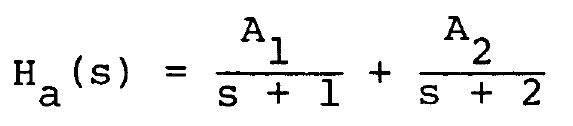
\includegraphics[width=0.3\linewidth]{img/img10}
		\end{figure}
	
		dimana
		
		\begin{figure}[H]
			\centering
			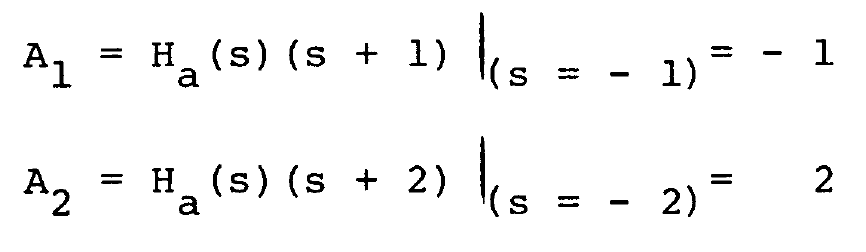
\includegraphics[width=0.5\linewidth]{img/img11}
		\end{figure}
		
		maka
		
		\begin{figure}[H]
			\centering
			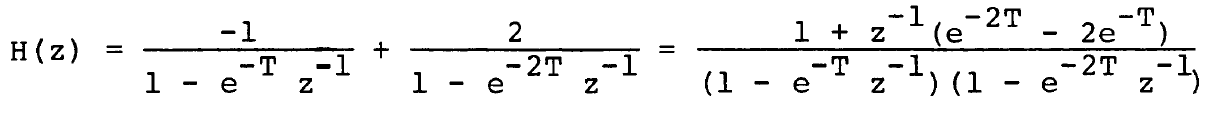
\includegraphics[width=\linewidth]{img/img12}
		\end{figure}
	
	\end{enumerate}
\end{document}